\documentclass[11pt,a4paper,twoside,openright]{report}
%\usepackage{hyperref}
\usepackage[pdftex]{graphicx} % Biblioteca para uso de figuras
\usepackage{color}

\graphicspath{{images/}}

\usepackage[brazil]{babel} % Biblioteca para uso da l�ngua portuguesa
\usepackage[T1]{fontenc} % Biblioteca para uso da acentua��o de entrada
\usepackage[latin1]{inputenc} % Biblioteca para uso da acentua��o de sa�da
\usepackage{textcomp}
\usepackage{lmodern}

\usepackage{amsthm,amsfonts,amsmath,amssymb}  % Biblioteca para uso de comandos matem�ticos
\usepackage{pslatex}
\usepackage{pstricks,pst-node,color,pst-gantt,pst-coil}
\usepackage{scalefnt}
\usepackage{float} %Permite colocar "\begin{figure}[H]" e colocar imagem exatamente onde desejar
\usepackage[hyphens]{url} % Para Aceitar URL nas referencias
\usepackage{pdfpages}

\usepackage{eurosym} %Pacote para possibilitar o uso do s�mbolo de euro "\euro"

\usepackage{listings} % para importa��o de c�digos fonte 

\usepackage[pdftex]{hyperref}
\hypersetup{bookmarks = true, % mostra a barra de bookmarks
	pdftitle = {O titulo do seu Trabalho}, % titulo
	pdfauthor = {Evandro L. L. Rodrigues}, % autor
	pdfsubject = {TCC}, % subject of the document
	pdfkeywords = {Sistemas Embarcados, ARM, Linux Embarcado}, % keywords
	colorlinks = true, 
	linkcolor = black,  
	citecolor = black,
	urlcolor = blue
}


\usepackage{comment}
\usepackage[margin=2.7cm]{geometry}
\renewcommand{\baselinestretch}{1.5}

\setlength{\parskip}{0em}

% Pacote para configurar cabe�alho e rodape
\usepackage{fancyhdr}
\pagestyle{empty}
\fancyhf{} % clear all header and footer fields

\fancypagestyle{plain}{\pagestyle{fancy}}
\renewcommand{\headrulewidth}{0pt}
\renewcommand{\footrulewidth}{0pt}


%Pacote para organizar apendices 
\usepackage[titletoc,toc]{appendix}
\renewcommand{\appendixtocname}{Ap�ndices}


\newenvironment{poliabstract}[1]
  {\renewcommand{\abstractname}{#1}\begin{abstract}}
  {\end{abstract}}

%%%%%%%%%%%%%%%%%%%%%%%%%%%%%%%%%%%%%% CONFIGURA��ES DE P�GINA %%%%%%%%%%%%%%%%%%%%%%%%%%%%%%%%%%%%%%
%\topmargin -2.1cm
%\oddsidemargin 0.5cm 
%\evensidemargin 0.5cm 
%\textwidth 15cm
%\textheight 25.1cm
	
%%%%%%%%%%%%%%%%%%%%%%%%%%%%%%%%%%%%%%%% IN�CIO DO DOCUMENTO %%%%%%%%%%%%%%%%%%%%%%%%%%%%%%%%%%%%%%%%
\begin{document}
	
%%%%%%%%%%%%%%%%%%%%%%%%%%%%%%%%%%%%%%  INCLUDES %%%%%%%%%%%%%%%%%%%%%%%%%%%%%%%%%%%%%%

%%%%%%%%%%%%%%%%%%%%%%%%%%%%%%%%%%%%%% ELEMENTOS PR�-TEXTUAIS %%%%%%%%%%%%%%%%%%%%%%%%%%%%%%%%%%%%%%
%%%%%%%%%%%%%%%%%%%%%%%%%%%%%%%%%%%%%%% CONFIGURA??ES DE CAPA %%%%%%%%%%%%%%%%%%%%%%%%%%%%%%%%%%%%%%%
\begin{titlepage}
	
	% CAPA PRINCIPAL
	\begin{center}
		\Huge{UNIVERSIDADE DE S�O PAULO}\\
		\vspace{0.02\textheight}
		\huge{ESCOLA DE ENGENHARIA DE S�O CARLOS}\\
		\vspace{0.01\textheight}
		\huge{DEPTO. DE ENGENHARIA EL�TRICA E DE COMPUTA��O}\\
		\vspace{0.2\textheight}
		\huge{\textbf{SEL0630 - Aplica��o de Microprocessadores II}}\\
		\vspace{0.05\textheight}
		\huge{\textbf{T�tulo do Trabalho}}
		\vspace{0.05\textheight}
	\end{center}
		{
			\begin{flushleft}
			\Large{ \textbf{Autor}: \hspace{1cm} Nome Aluno, n$^o$. USP 0000000 }\\
			\Large{ \textbf{Autor}: \hspace{1cm} Nome Aluno, n$^o$. USP 0000000 }\\
			\Large{ \textbf{Orientador}: \hspace{0.3cm} Prof. Dr. Evandro Luis Linhari Rodrigues }\\
			\end{flushleft}
	
			\begin{center}
				\vspace{0.09\textheight}
				\Large{S�o Carlos}\\
				\Large{2017}
			\end{center}
		}
	
\end{titlepage}


%%%%%%%%%%%%%%%%%%%%%%%%%%%%%%%%%%%%%%%%%%%%%%% INSER??O P?GINA EM BRANCO %%%%%%%%%%%%%%%%%%%%%%%%%%%%%%%%%%%%%%%%%%%%%%
\cleardoublepage


%%%%%%%%%%%%%%%%%%%%%%%%%%%%%%%%%%%%%%%%%%%%%%% RESUMO - PORTUGUES %%%%%%%%%%%%%%%%%%%%%%%%%%%%%%%%%%%%%%%%%%%%%%
\
\vspace{0.11\textheight} 

\begin{center}
\textbf{\Huge{Resumo}}
\end{center}

\vspace{0.05\textheight}
			
Texto em \underline{\textbf{UM PAR�GRAFO}} apenas - deve conter \underline{tudo} resumidamente (introdu��o, m�todo(s), resultados e conclus�es), de tal forma que seja poss�vel compreender a proposta e o que foi alcan�ado.


\vspace{0.05\textheight}
	
Palavras-Chave: palavra1, palavra2, palavra3, palavra4, palavra5.

%%%%%%%%%%%%%%%%%%%%%%%%%%%%%%%%%%%%%%%%%%%%%%% INSER??O P?GINA EM BRANCO %%%%%%%%%%%%%%%%%%%%%%%%%%%%%%%%%%%%%%%%%%%%%%
\cleardoublepage

%%%%%%%%%%%%%%%%%%%%%%%%%%%%%%%%%%%%%%%%%%%%%%% RESUMO - INGL�S %%%%%%%%%%%%%%%%%%%%%%%%%%%%%%%%%%%%%%%%%%%%%%
\
\vspace{0.11\textheight} 

\begin{center}
\textbf{\Huge{Abstract}}
\end{center}

\vspace{0.05\textheight}	
		
Abstract, abstract, abstract, abstract, abstract, abstract, abstract, abstract, abstract, abstract, abstract, abstract, abstract, abstract, abstract, abstract, abstract, abstract, abstract, abstract, abstract, abstract, abstract, abstract, abstract, abstract, abstract, abstract, abstract, abstract, abstract, abstract, abstract, abstract, abstract, abstract, abstract, abstract, abstract, abstract, abstract, abstract, abstract.

\vspace{0.05\textheight}

Keywords: keyword1, keyword2, keyword3, keyword4, keyword5.

%%%%%%%%%%%%%%%%%%%%%%%%%%%%%%%%%%%%%%%%%%%%%%% INSER??O P?GINA EM BRANCO %%%%%%%%%%%%%%%%%%%%%%%%%%%%%%%%%%%%%%%%%%%%%%
\cleardoublepage
%\thispagestyle{empty}
%\newpage
%%%%%%%%%%%%%%%%%%%%%%%%%%%%%%%%%%%%%%%%%%%%%%% RESUMO %%%%%%%%%%%%%%%%%%%%%%%%%%%%%%%%%%%%%%%%%%%%%

%%%%%%%%%%%%%%%%%%%%%%%%%%%%%%%%%%%%% CONFIGURA??ES DOS ?NDICES %%%%%%%%%%%%%%%%%%%%%%%%%%%%%%%%%%%%%
%\clearpage
%\thispagestyle{empty}
\listoffigures % ?ndice de Figuras
(Se houver...)
\listoftables % ?ndice de Tabelas
(Se houver...)
%%%%%%%%%%%%%%%%%%%%%%%%%%%%%%%%%%%%%%%%%%%%%%% INSER??O P?GINA EM BRANCO %%%%%%%%%%%%%%%%%%%%%%%%%%%%%%%%%%%%%%%%%%%%%%
\cleardoublepage

%%%%%%%%%%%%%%%%%%%%%%%%%%%%%%%%%%%%% LISTA DE ABREVIATURAS %%%%%%%%%%%%%%%%%%%%%%%%%%%%%%%%%%%%%
\

\vspace{0.11\textheight} 

\textbf{\Huge{Siglas}}
(Se houver...)
\vspace{0.05\textheight}
			
\begin{tabbing}
\hspace*{0.5cm}\=\hspace{2.5cm}\= \kill

% Exemplo de lista de lista de abreviaturas
\> MVC \> \textit{Model-View-Controller} - Modelo-Vis�o-Controlador \\
\> POO \> Programa��o Orientada a Objetos \\
\> UI \>  \textit{User Interface} - Interface do Usu�rio \\
\> UML \> \textit{Unified Modeling Language} - Linguagem de Modelagem Unificada \\


\end{tabbing}
\cleardoublepage
%%%%%%%%%%%%%%%%%%%%%%%%%%%%%%%%%%%%% CONFIGURA��ES DOS �NDICES %%%%%%%%%%%%%%%%%%%%%%%%%%%%%%%%%%%%%
%\usepackage{fancyhdr}
\pagestyle{fancy}
\fancyhf{} % clear all header and footer fields
\fancyhead[RO, LE] {\thepage}

\fancypagestyle{plain}{\pagestyle{fancy}}

\tableofcontents % �ndice Geral

%%%%%%%%%%%%%%%%%%%%%%%%%%%%%%%%%%%%%%%% ADI��O DOS CAP�TULOS %%%%%%%%%%%%%%%%%%%%%%%%%%%%%%%%%%%%%%%	
\chapter{Introdu��o}
\label{Introducao}

\par A L�ngua Brasileira de Sinais (Libras) � reconhecida oficialmente desde 2002 por meio da lei N� 10.436 (regulamentada pelo decreto N�5.626 de 2005). Este marco representa um grande avan�o para a comunidade surda, que possuem agora uma l�ngua pr�pria e direitos garantidos por lei, como expresso nos artigos 2�, 3� e 4� das obriga��es do governo em divundir a Libras e garantir o atendimento e tratamento � comunidade surda~\cite{Benassi}.
\par Segundo o Portal Brasil, existem mais de 9,7 milh�es de surdos no pa�s (dados do Censo de 2010), no entanto, a acessibilidade para essas pessoas ainda � um desafio devido a falta de int�rpretes~\cite{PortalBrasil}. No intuito de diminuir as barreiras de comunica��o, v�rios aplicativos tem surgido com a proposta de traduzir sites, textos e at� mesmo voz para a Libras, como � o caso do ProDeaf e do Hand Talk apenas para citar alguns. No entanto, o processo inverso de tradu��o, ou seja, de Libras para o portugu�s, n�o � uma funcionalidade muito comum nestes aplicativos.
\par Na tentativa de criar uma interface entre surdos e ouvintes, busca-se neste trabalho desenvolver um aplicativo capaz de reconhecer gestos em Libras. Para este trabalho, o foco ser� dado na interpreta��o de sinais est�ticos, mais especificamente na identifica��o dos n�meros.
% (em junho de 2017, foi lan�ado o projeto Giulia para Android, o primeiro aplicativo com esta funcionalidade para Libras).

%Introdu��o do trabalho.
% 
%\par Na reda��o da monografia, que � parte important�ssima do projeto, pois � aquela que ficar� p�blica, precisamos definir muito bem o t�tulo, construir um Resumo com todas as partes de um Resumo, esclarecer o(s) objetivo(s) e construir uma conclus�o completa, tudo isso quase que ao mesmo tempo, pois o trabalho j� terminou.
%A Introdu��o deve conter um hist�rico (com muitas refer�ncias atuais-procure nas bases consagradas, como por exemplo IEEE, para apresentar n�o s� refer�ncias vol�teis-aquelas da Internet) do assunto apontando a origem e os avan�os que est�o publicados, ressaltando o "foco" de ataque do projeto.
%Depois, compor um bom Embasamento Te�rico citando as refer�ncias de onde est� o assunto todo de cada t�pico (sem se confundir com a apresenta��o dos materiais usados no projeto), pois � o lugar onde estar�o presentes as partes da ci�ncia ou as t�cnicas de forma geral que foram utilizadas para construir a solu��o (exemplo: Sistemas Embarcados � um t�pico e n�o Raspberry Pi, Linux Embarcado � um t�pico e n�o a distribui��o escolhida, por�m Linux � um subt�pico de Sistemas Operacionais). Depois mostrar Material e M�todos, ou Desenvolvimento do Projeto, mostrando logo na entrada do cap�tulo uma figura ou diagrama que apresente de forma geral como as partes est�o relacionadas/conectadas. Mostrar os algoritmos da solu��o em forma de fluxogramas ou usando UML, de maneira clara e completa. Se for necess�rio apresentar trechos de c�digo para ressaltar solu��es ou apresentar abordagens, tamb�m que seja de forma direta e simplificada. C�digos completos dever�o estar nos Ap�ndices para a Monografia final, depois da defesa.  
%Assim, consegue-se mostrar o quanto voc� evoluiu com os aprendizados do curso e com aqueles que voc� buscou a mais, e o quanto tem de solu��o legal e atual na sua proposta. 
%Valorize as conquistas alcan�adas apresentando e discutindo os resultados com gr�ficos, tabelas, figuras, etc.
%Nas Conclus�es, tamb�m n�o esque�a de apontar as defici�ncias ou limita��es que s�o inerentes ao trabalho e que no momento n�o est�o no(s) objetivo(s), e tamb�m as defici�ncias ou limita��es dos procedimentos que vc incorporou ao seu trabalho de outros autores.
%Indique as dire��es para os trabalhos futuros, pois o autor conhece como ningu�m as oportunidades de continuidade e avan�os do trabalho.
%
%Exemplo de cita��o de Refer�ncia \cite{referencia1}. Outra refer�ncia para a bibliografia \cite{referencia2}.
%
%Segundo \cite{referencia3} h� uma sequ�ncia l�gica para a reda��o da monografia como apresenta em \cite{enzo}.
%
%Refer�ncia para a figura \ref{logo}.
%
% \begin{figure}[H]
% 	\centering
% 	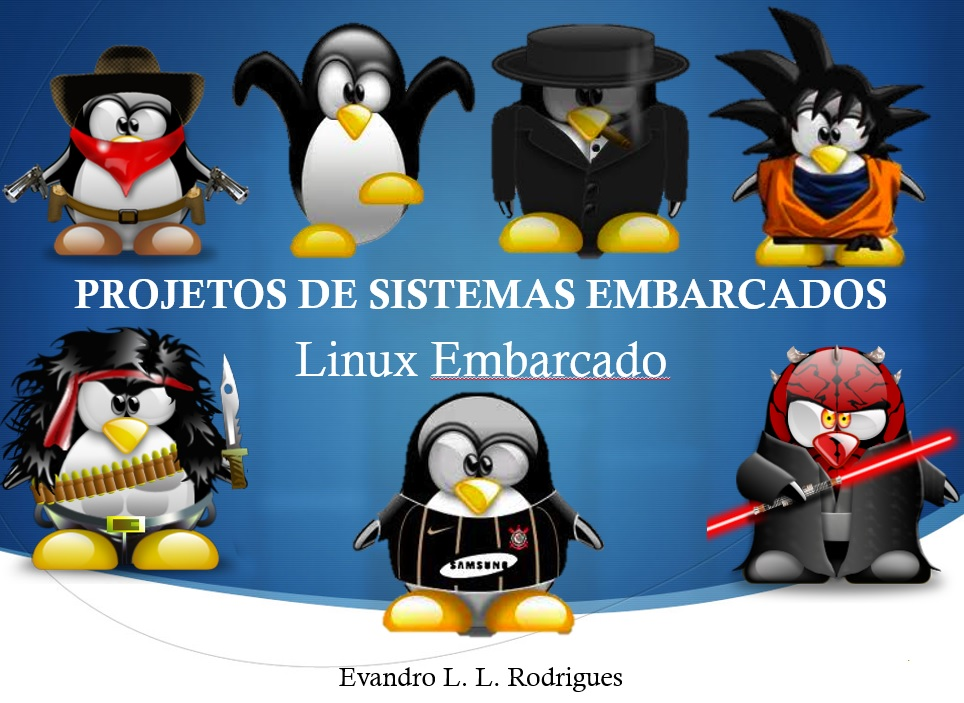
\includegraphics[scale=0.35]{./Resources/proj_sistemas_embarcados.jpg}
% 	\caption{Logo da Disciplina.}
% 	\label{logo}
% \end{figure}

% % % % % % % % % % % % % % % % % % % % % % % % % % % % % % % % % % % % % % % % % % % % % % % % % % %
\section{Motiva��o}

\par � vasta a quantidade de estudos envolvendo o reconhecimento de gestos aplicadas � l�nguas de sinais. Tamb�m � vasta a cole��o de aplicativos dispon�veis para traduzir o portugu�s para Libras. No entanto, sistemas capazes de fazer o processo inverso de tradu��o e que est�o dispon�veis � sociedade ainda s�o escassos.
\par A grande motiva��o do trabalho � atuar de forma a fornecer ferramentas para que um usu�rio de Libras possa interagir com pessoas que n�o tem conhecimento da l�ngua de sinais.
% % % % % % % % % % % % % % % % % % % % % % % % % % % % % % % % % % % % % % % % % % % % % % % % % % %
\section{Objetivo}

\par Este trabalho tem como objetivo principal o desenvolvimento de um sistema para interpreta��o de sinais em Libras, focando na identifica��o dos n�meros de 0 a 7.


% % % % % % % % % % % % % % % % % % % % % % % % % % % % % % % % % % % % % % % % % % % % % % % % % % %
\section {Justificativa}

 
\par O trabalho se justifica por atuar de forma a buscar alternativas � falta de int�rpretes dispon�veis aos usu�rios de Libras, n�o com o intuito de substitu�-los, mas na tentativa de aumentar a autonomia de pessoas surdas.


% % % % % % % % % % % % % % % % % % % % % % % % % % % % % % % % % % % % % % % % % % % % % % % % % % %
\section {Organiza��o do Trabalho}

Este trabalho est� distribu�do em XXX cap�tulos, incluindo esta introdu��o, dispostos conforme a descri��o que segue:

Cap�tulo 2: Descreve .....................................................................................

Cap�tulo 3: Discorre sobre .....................................................................................

Cap�tulo 4: Apresenta .....................................................................................




























%\chapter{Especifica��o do Projeto}
\label{Especificacao}

Especifica��o do projeto.


% % % % % % % % % % % % % % % % % % % % % % % % % % % % % % % % % % % % % % % % % % % % % % % % % % %
\section{Se��o 1}

Se��o dentro de um cap�tulo. 



% % % % % % % % % % % % % % % % % % % % % % % % % % % % % % % % % % % % % % % % % % % % % % % % % % %
\section{Se��o 2}

Outra se��o dentro do cap�tulo.


\chapter{Embasamento Te�rico ou Fundamenta��o Te�rica}
\label{EmbasamentoTeorico}

Embasamento te�rico para o desenvolvimento do trabalho.

Leia o texto que est� na Introdu��o e as dicas mais � frente...





\chapter{Materiais e M�todo}
%\label{Introducao}



% % % % % % % % % % % % % % % % % % % % % % % % % % % % % % % % % % % % % % % % % % % % % % % % % % %
\section{Material}
%\par Com a inten��o de solucionar um problema do mundo real e facilitar vidas no que diz respeito � acessibilidade, de maneira a realmente otimizar de alguma forma o mundo das pessoas envolvidas, surgiu a id�ia de desenvolver um sistema para que quem tenha defici�ncia auditiva possa se comunicar com outros que desconhecem a linguagem para surdos mudos, j� que esta � pouco difundida e ensinada, trazendo desta forma melhorias para os deficientes em sua desenvoltura pessoal, vida profissional e educa��o, al�m de incentivar a aprendizagem da LIBRAS. 
%
%\par O Projeto base tem por objetivo estruturar e desenvolver um sistema de interpreta��o dos n�meros do alfabeto da LIBRAS de 0 a 7.

\par O projeto principal consiste em um aplicativo Android conectado a um sistema embarcado em uma Raspberry Pi (com Raspian) em rede e com comunica��o \textit{web} para um \textit{website} para treinamento dos s�mbolos. Ou seja, generalizando a divis�o do projeto, tem-se os seguintes materiais envolvidos:

\begin{itemize}
	\item Android Studio (3.0.1): para a cria��o do aplicativo, o qual processa as imagens da c�mera do \textit{smartphone} para transferi-las � Raspberry pi.
	
	\item Raspberry Pi (modelo B): microcomputador embarcado, com uma distribui��o Linux e programado para as necessidades do projeto.
	\item Raspian (4.9.35): distrubui��o variante do Debian do Linux baseada na arquitetura ARM do hardware da Raspberry Pi.
	\item Python 3: linguagem de programa��o interpretada de alto n�vel utilizada durante toda execu��o do projeto, tanto para rotinas internas de classifica��o, quanto para cria��o do \textit{website}.
	\item Flask (0.12.2): \textit{framework} leve e poderoso para Python, utilizada na cria��o do sistema \textit{web}.
	\item OpenCV (3.3): significando \textit{Open Source Computer Vision Library}, � uma biblioteca multiplataforma utilizada no aplicativo Android afim de processar as imagens obtidas na c�mera.
	
	\item Materilize (v0.100.2): \textit{framework} para customiza��o da interface \textit{web}.
	\item MongoDB (2.4.10): modelo de banco de dados \textit{NoSQL}, o que facilita sua crian��o, servindo como armazenamento das imagens dos s�mbolos para posteriores compara��es e classifica��es.
	
\end{itemize}

%\par O sistema e suas comunica��es, em resumo, funcionam da seguinte maneira: O aplicativo Android � respons�vel por adquirir a imagem via c�mera do \textit{Smartphone}, conta em sua implementa��o com OpenCV (Open Source Computer Vision Library) para interpretar as imagens, detectando bordas, pele e face, envia ent�o essas imagens de modo simult�neo para o sistema rodando na Raspiberry


% % % % % % % % % % % % % % % % % % % % % % % % % % % % % % % % % % % % % % % % % % % % % % % % % % %
\section{M�todo}

\par O m�todo utilizada para realizar este trabalho baseia-se no que foi utilizado em~\cite{Barros},~\cite{Yeo} e~\cite{Chen}. Basicamente o processo se divide conforme mostra a figura~\ref{fig:processo}.

\begin{figure}[H]
	\centering
	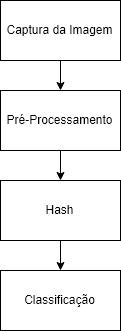
\includegraphics[width=0.2\textwidth]{./Resources/procedimento.png}
	\caption{M�todo utilizado.}
	\label{fig:processo}
\end{figure}

\subsection{Captura da Imagem}

\par A captura da imagem � feita pela c�mera do aparelho Android. N�o foi imposta nenhuma restri��o quanto �s caracter�sticas da c�mera para este projeto.

\subsection{Pr�-Processamento}

\par O pr�-processamento � realizado com aux�lio da biblioteca \textit{OpenCV} e consiste em tratar a imagem capturada pela c�mera de modo isolar as caracter�sticas desejadas (neste caso, busca-se isolar a regi�o das m�os).

\par O processo de pr�-processamento � mostrado na figura~\ref{fig:pre_proc}. S�o realizadas 3 etapas de maneira independente:

\begin{itemize}
	\item Detec��o de bordas: foi utilizado o detector de bordas de \textit{Canny}, por meio da fun��o \textit{Imgproc.Canny}. 
	\item Detec��o de face: utiliza o \textit{CascadeClassifier} da biblioteca \textit{OpenCV} para fazer a detec��o da regi�o quadrada que cont�m uma face. Esta regi�o � ent�o preenchida (preto) de modo a eliminar a face da imagem.
	\item Detec��o de pele: detecta regi�es dentro de uma faixa de cores (utilizando o espa�o HSV). O ajuste para detec��o de pele foi feito manualmente.
\end{itemize}

\begin{figure}[H]
	\centering
	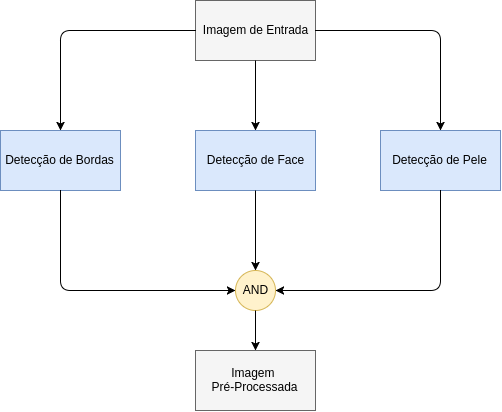
\includegraphics[width=0.7\textwidth]{./Resources/pre_processamento.png}
	\caption{Etapas do pr�-processamento.}
	\label{fig:pre_proc}
\end{figure}

\par Ao final, o resultado dos 3 processos s�o combinados em uma �nica imagem. O resultado � uma imagem como mostrado na figura~\ref{fig:imagem_pre_proc}, onde apenas o contorno das m�os fica vis�vel na tela. Esta � imagem � convertida para "jpg" e enviada pela rede � Raspberry onde ocorrer� a segunda parte do processo.

\begin{figure}[H]
	\centering
	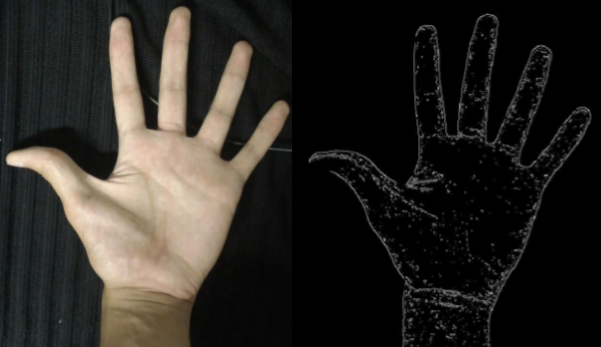
\includegraphics[width=0.7\textwidth]{./Resources/mao_transformada.png}
	\caption{Resultado do pr�-processamento.}
	\label{fig:imagem_pre_proc}
\end{figure}

\subsection{\textit{Hash}}

\par A imagem recebida passa pelo processo de \textit{Average Hash}, disponibilizado pela biblioteca \textit{ImageHash} do Python. Este processo � feito para facilitar a compara��o das imagens pois, ao final do processo, as imagens ser�o representadas por n�meros, que podem ser facilmente armazenadas na base de dados e comparada com opera��es aritm�ticas simples.

\par Experimentalmente, chegou-se ao valor de 256-bits para o tamanho do \textit{hash}, abaixo deste valor n�o era poss�vel diferenciar as imagens com o classificador utilizado. A figura~\ref{fig:exemplo_hash} mostra um exemplo de como o \textit{hash} atua na imagem binarizada mostarda na figura~\ref{fig:imagem_pre_proc}.

\begin{figure}[H]
	\centering
	
\includegraphics[width=0.7\textwidth]{./Resources/Hash_mao.png}
	\caption{\textit{Hash} de 64 bits aplicado na imagem binarizada.}
	\label{fig:exemplo_hash}
\end{figure}

\subsection{Classifica��o}

\par Por meio da interface \textit{web} desenvolvida, mostrada na figura~\ref{fig:website}, � poss�vel visualizar cada imagem recebida pela Raspberry e fazer o treinamento do banco de dados relacionando a imagem visualizada ao seu n�mero correspondente.

\begin{figure}
	\centering
	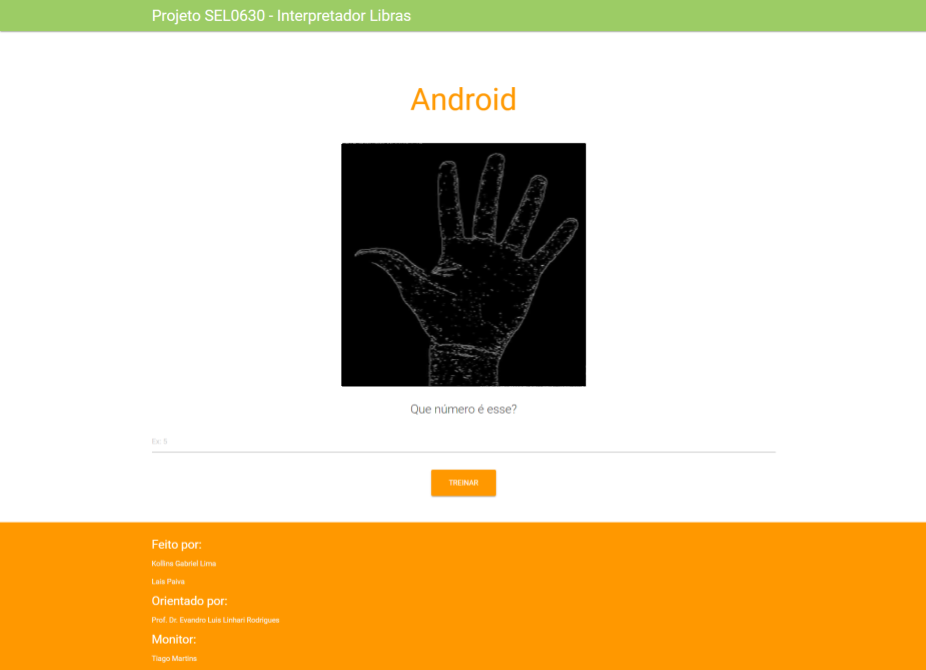
\includegraphics[width=0.7\textwidth]{./Resources/pagina_treinamento.png}
	\caption{P�gina \textit{web} para treinamento do banco de dados.}
	\label{fig:website}
\end{figure}

\par Ao mesmo tempo, em segundo plano, o classificador \textit{k-NN} executa continuamente a classifica��o de cada imagem recebida. Foram utilizados os 3 resultados melhores classificados (3 vizinhos). Este valor tamb�m foi decidido experimentalmente de forma a n�o consumir muito tempo no processo de classifica��o.

\par Antes de enviar o resultado novamente ao Android, foi aplicado um \textit{threshold} buscando diminuir a taxa de erro. Desta forma, cada novo resultado obtido do classificador s� � enviado pela rede como resultado final se for, pelo menos, 10\% diferente do resultado enviado anteriormente. O valor de 10\% foi obtido verificando como o classificador se comporta quando n�o h� mudan�a no s�mbolo de entrada (qual o erro nesta condi��o).

\par A imagem~\ref{fig:diagrama_completo} apresenta um diagrama simplificado do funcionamento do sistema como um todo.

\begin{figure}
	\centering
	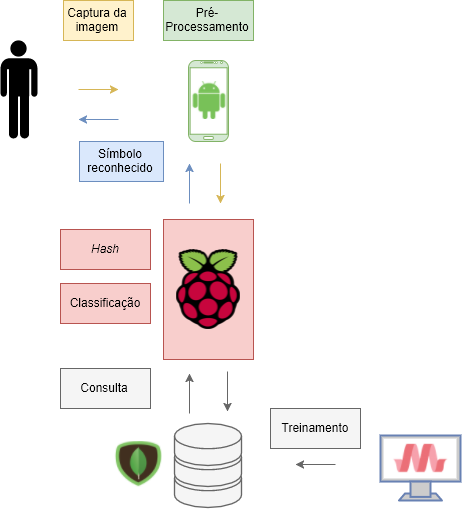
\includegraphics[width=\textwidth]{./Resources/diagrama_completo_micros2.png}
	\caption{Diagrama simplificado do sistema.}
	\label{fig:diagrama_completo}
\end{figure}

\newpage
\par Os c�digos desenvolvidos para esta aplica��o podem ser encontrados no Github.

\begin{itemize}
	\item Android: \url{https://github.com/kollinslima/ProjetoFinal_micros2_android} 
	\item Raspberry: \url{https://github.com/kollinslima/ProjetoFinal_micros2_rasp.git}
\end{itemize}
\chapter{Resultados e Discuss�es}
\label{Resultados}

\par Os s�mbolos num�ricos a serem classificados s�o mostrados na figura~\ref{fig:simbolos}.

\begin{figure}
	\centering
	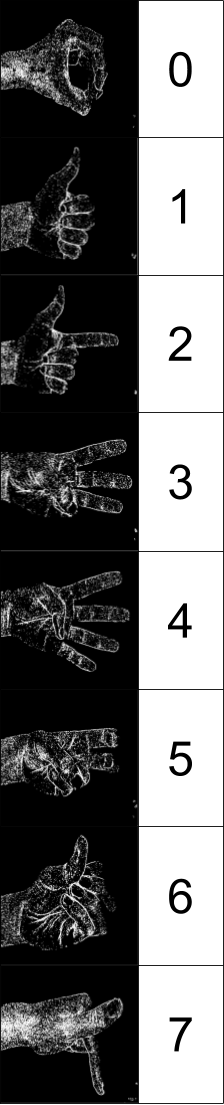
\includegraphics[height=\textheight]{./Resources/Maos_numeros.png}
	\caption{S�mbolos propostos para o sistema de classifica��o.}
	\label{fig:simbolos}
\end{figure}

\par O sistema funciona com baixas taxas de erro quando trabalha com poucos s�mbolos, no entanto o processo de classifica��o se torna impreciso conforme a quantidade de s�mbolos diferentes aumenta. A figura~\ref{fig:erro} mostra a taxa de erro obtida em fun��o da quantidade de s�mbolos diferentes que foram adicionados ao banco de dados.

\begin{figure}[H]
	\centering
	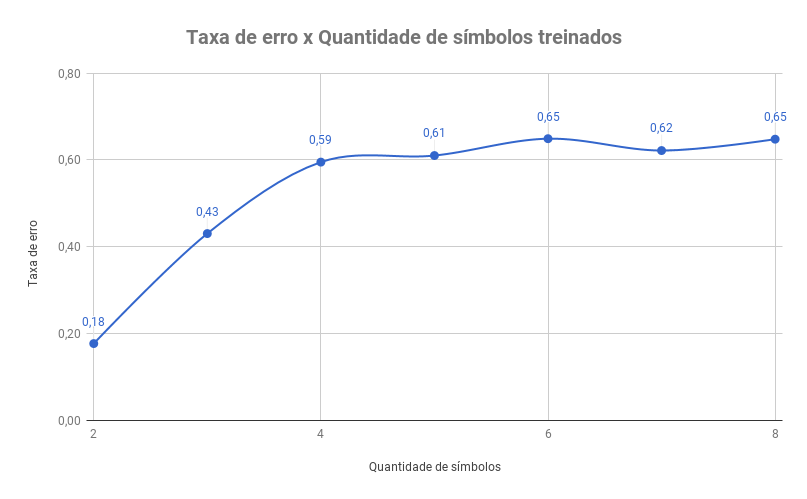
\includegraphics[width=\textwidth]{./Resources/grafico_erro.png}
	\caption{Diagrama simplificado do sistema.}
	\label{fig:erro}
\end{figure}

\par Para realizar os testes, o banco de dados foi treinado com a mesma quantidade de exemplos para cada s�mbolo (3 exemplos) e foi dada como entrada a mesma quantidade de inst�ncias de cada s�mbolo (3 inst�ncias para cada s�mbolo treinado). O gr�fico apresenta a taxa de desequil�brio entre o esperado e o obtido.

\par Como mostardo na figura~\ref{fig:erro}, acima de 2 s�mbolos o sistema � ca�tico, com baixas taxas de acerto. Esse resultado indica duas possibilidades para que o sistema n�o funcione como o esperado:
\begin{enumerate}
	\item O processo de \textit{hash} elimina muitas caracter�sticas da imagem de forma que diferenciar muitas imagens se torna uma tarefa complicada.
	\item O classificador utilizado (\textit{k-NN}) n�o � bom o suficiente para classificar muitos s�mbolos.
\end{enumerate}

\par Muito embora o classificador \textit{k-NN} seja bastante simples se comparado �s t�cnicas utilizadas nos trabalhos citados anteriormente, a transforma��o \textit{hash} � a principal respons�vel pelos resultados obtidos, uma vez que caracter�sticas importantes da imagem s�o descartadas neste processo.
\par Isso ficou evidente em um segundo teste realizado com um novo conjunto de s�mbolos, mostrados na figura~\ref{fig:novos_simbolos}. Como se pode notar, estes novos s�mbolos possuem um n�vel de detalhamento menor e exploram diferentes regi�es da imagem, o que faz com que o \textit{hash} de cada imagem tenha uma maior diferen�a.

\begin{figure}
	\centering
	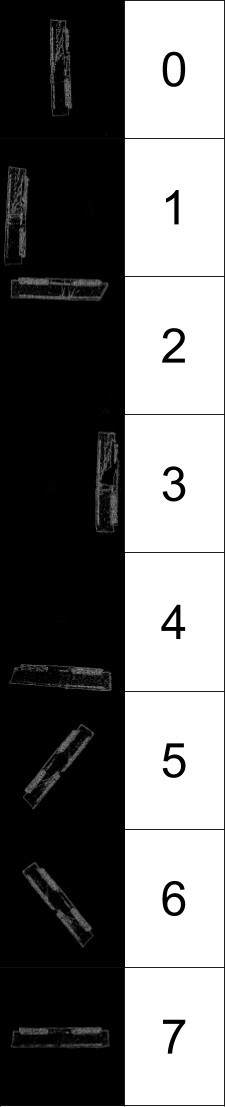
\includegraphics[height=\textheight]{./Resources/novos_numeros.png}
	\caption{S�mbolos alternativos para o sistema de classifica��o.}
	\label{fig:novos_simbolos}
\end{figure}

\par Com estes novos s�mbolos, obteve-se uma melhora na classifica��o de aproximadamente 10\% (em rela��o ao caso de teste com 8 s�mbolos). Embora essa taxa de erro ainda seja elevada (acima de 50\%), na pr�tica p�de-se notar um sistema muito mais est�vel e preciso quando comparado ao caso de teste anterior.


\chapter{Conclus�o}
\label{Conclusao}

\par Neste trabalho foi apresentado uma proposta para realizar o reconhecimento da linguagem de sinais, aplicada � L�ngua Brasileira de Sinais - LIBRAS, atrav�s de um sistema Android .

\par Pode-se dizer que o trabalho atinge parcialmente seus objetivos. Por um lado, foi implementado um sistema capaz de ler, processar, classificar e responder textualmente os s�mbolos apresentados por meio da c�mera de um \textit{smartphone} Android. Por outro, com uma taxa de erro superior � 60\%, o sistema n�o � capaz de fazer a classifica��o correta para todos os s�mbolos num�ricos propostos. 

\par Ademais, a grande quantidade de erros n�o permite que o sistema possa ser confi�vel e usado livremente como aplicativo comerci�vel e disponibilizado para download na comunidade Android, pois seu uso ainda n�o estaria finalizado com sucesso. Tamb�m foi identificado que o uso da biblioteca \textit{OpenCV} no aplicativo o tornou demasiado grande, e seu download implicaria na necessidade de complementar com o da biblioteca \textit{OpenCV}, o que traria desconfian�a ao usu�rio, al�m de que testes demonstraram que o aplicativo demandou bastante da bateria do \textit{smartphone}.

\par Analisando o que foi desenvolvido, notou-se que esta proposta n�o � suficiente para prover independ�ncia ao indiv�duo surdo, que � o objetivo principal, pois al�m de se limitar aos n�meros somente, o sistema n�o � f�cil uso no dia-a-dia, mesmo se estivesse em perfeito funcionamento, uma vez que depende de uma c�mera apontando para o usu�rio, fazendo com que o aplicativo dependesse de duas pessoas para seu uso (uma segurando a c�mera e outra fazendo os gestos), do contr�rio restringiria os movimentos por exigir que uma das m�os segure a c�mera. Seu uso seria mais eficiente em um contexto de palestra ou algum outro evento onde j� existe uma c�mera externa monitorando o ambiente, tamb�m com exemplo de pesquisa e desenvolvimento na �rea acessibilidade com processamento de imagens.

\par Apesar dos resultados obtidos, o desenvolvimento deste projeto exigiu conhecimento de diversas �reas antes pouco exploradas, o que foi de grande valia para o aprendizado. Entre os conhecimentos obtidos, pode-se destacar as diversas t�cnicas de processamento de imagem que foram necess�rias na etapa de pr�-processamento (com aux�lio da biblioteca \textit{OpenCV}); o uso da Raspberry-pi como elemento central no projeto e seu Linux Embarcado; o uso do \textit{Flask} para desenvolver a interface \textit{web}; o uso do banco de dados MongoDB al�m da pr�tica em desenvolvimento na linguagem Python e para Android.

\par Por fim, foi observado que para a conclus�o efetiva dos objetivos propostos e para benfeitoria dos deficientes auditivos o sistema ainda precisaria ser mais desenvolvido e trabalhado para chegar a um resultado mais utiliz�vel com bom desempenho, com esta an�lise foi poss�vel concluir que em trabalhos futuros, � preciso pensar em outras maneiras de fazer o reconhecimento de gestos, seja por um processamento de imagem diferente, como utilizar a biblioteca \textit{OpenCV} na Raspiberry-pi diretamente, ou uma melhor classifica��o das hashs, que traga uma resposta mais r�pida e assertiva ao sistema, que seja de f�cil uso por uma �nica pessoa e que n�o envolva uma quantidade excessiva de hardware externo, tanto para prover um sistema mais acess�vel, quanto devido � est�tica.


%\section*{Trabalhos futuros}
%
%Isso � para a Monografia Final de defesa.....












%%%%%%%%%%%%%%%%%%%%%%%%%%%%%%%%%%%%%% ADI��O DAS BIBLIOGRAFIAS %%%%%%%%%%%%%%%%%%%%%%%%%%%%%%%%%%%%%
\addcontentsline{toc}{chapter}{Refer�ncias}
\renewcommand{\bibname}{Refer�ncias}	
\bibliographystyle{unsrt} % Define o estilo da bibliografia
\bibliography{./Content/References} % Faz referencia ao arquivo ref.bib

%%%%%%%%%%%%%%%%%%%%%%%%%%%%%%%%%%%%%%%%%%% ADI��O DOS AP�NDICES %%%%%%%%%%%%%%%%%%%%%%%%%%%%%%%%%%%%%%%%	
%\begin{appendices}
%	%\appendix
%	\chapter{Cuidados e orienta��es para a elabora��o de texto}
\label{Ap�ndice Ap�ndice A}

\begin{center}
\textbf {\color{blue}{Dicas para a reda��o de uma boa monografia de TCC}}
\end{center}

Observe as diretrizes no site do Depto.
\begin{center}
	\href{http://143.107.182.35/sel/files\_EE/tcc\_-\_diretrizes\_EESC\_v\_2010.pdf}{http://143.107.182.35/sel/files\_EE/tcc\_-\_diretrizes\_EESC\_v\_2010.pdf}
\end{center}

Veja no Portal de Livros Abertos da USP as mais novas vers�es das Diretrizes para apresenta��o de disserta��es e teses da USP.
\begin{itemize}
	\item Parte I (ABNT) - \href{http://dx.doi.org/10.11606/9788573140606}{http://dx.doi.org/10.11606/9788573140606}
	\item Parte II (APA) - \href{http://dx.doi.org/10.11606/9788573140576}{http://dx.doi.org/10.11606/9788573140576}
	\item Parte III (ISO) - \href{http://dx.doi.org/10.11606/9788573140590}{http://dx.doi.org/10.11606/9788573140590}
	\item Parte IV (Vancouver) - \href{http://dx.doi.org/10.11606/9788573140569}{http://dx.doi.org/10.11606/9788573140569}
\end{itemize}



Observe os elementos pr�-textuais neste documento....tem uma sequ�ncia a ser seguida (Capa, contracapa, Ficha catalogr�fica para a vers�o final, Listas de Figuras, Tabelas e S�mbolos/Abreviaturas).\\

\textbf{Resumo/abstract}\\
Texto em \underline{\textbf{um}} par�grafo apenas. Deve conter \underline{tudo} resumidamente (introdu��o, m�todo(s), resultados e conclus�es), de tal forma que seja poss�vel compreender a proposta e o que foi alcan�ado;\\
Palavras-chave: Logo abaixo do Resumo/Abstract.\\

\textbf{Cap�tulo 1} - Introdu��o\\
Realmente introduz o leitor indicando quais s�o as dire��es do trabalho ? Apresenta o tema e o objeto do trabalho e cont�m as Refer�ncias do Estado da arte (quem est� fazendo e em que n�vel os trabalhos da �rea est�o hoje)?\\
- Justificativa/relev�ncia do trabalho: explana��o sobre porque o trabalho se justifica e quais os pontos de relev�ncia do mesmo;\\
- Objetivo(s): \textbf{"\underline{somente}"} o(s) objetivo(s) em uma frase. Tamb�m podem ser descritos na forma de "gerais" \ e/ou "espec�ficos";\\
- Organiza��o do trabalho (o que tem em cada cap�tulo).\\

N�o h� necessidade de reproduzir (copiar) as obras que embasam o trabalho e sim colocar o suficiente para o entendimento do trabalho e citar as refer�ncias;

\textbf{Cap�tulo 2} - Embasamento Te�rico ou Fundamenta��o Te�rica\\
Revis�o da literatura dos t�picos  que sustentam a ci�ncia e o conhecimento, relativos ao(s) objetivo(s) e o(s) m�todo(s) escolhido(s) para o desenvolvimento do trabalho;

\textbf{Cap�tulo 3} - Material e M�todos ou Desenvolvimento do Projeto\\
Descri��o clara dos procedimentos e do material adotados para o desenvolvimento do trabalho (\underline{sem resultados}), incluindo sua adequa��o ao trabalho.\\ 
Tem que responder �s perguntas:\\
- Est� com tamanho adequado (proporcional) � monografia? \\
- H� informa��o suficiente e clara sobre os materiais e sobre os m�todos  adotados?\\
N�o h� necessidade de reproduzir (copiar) as obras que embasam o trabalho e sim colocar o suficiente para o entendimento do trabalho e citar as refer�ncias.

\textbf{Cap�tulo 4} - Resultados/Discuss�es\\
Aqui se mostra o que o trabalho permitiu produzir, e �s vezes o que pode ser comparado com outros trabalhos - aqui ficam claras se as propostas do trabalho s�o relevantes ou n�o, pois devem permitir a discuss�o do trabalho. 

Deve responder: Os resultados est�o claros em bom n�mero (nem muito nem pouco) que permitam avaliar realmente a proposta e o que foi produzido?

\textbf{Cap�tulo 5} - Conclus�es\\
"Fecham" com os objetivos? (respondem aos objetivos?) - aqui � que "se vende o peixe"  pois ir�o valorizar (ou n�o) o trabalho realizado. Normalmente � uma parte do trabalho "um pouco desprezada", pois o autor j� est� "cansado....". Mas aqui � um ponto importante de medida se o trabalho tem ou n�o valor.
 
\textbf{Refer�ncias}\\
Deve conter todas as refer�ncias {\color{red}{citadas no texto}}. Observar as Diretrizes, pois l� est�o os formatos corretos de cita��o.

\textbf{Ap�ndices}\\
Todo o material produzido pelo autor durante o trabalho, que o mesmo julga importante disponibilizar, mas que n�o deve estar no corpo do trabalho, pois atrapalharia a leitura do mesmo.

\textbf{Anexos}\\
Todo o material que n�o � de autoria pr�pria, mas que � importante para completar as informa��es do corpo do texto (ex. datasheet).\\


\begin{center}	
\underline{Outras observa��es \textbf{IMPORTANTES} (\color{red}{leia isso com aten��o})}
\end{center}

NUNCA copie texto de outro autor sem a devida forma de cita��o (ver em diretrizes); a c�pia configura pl�gio! Com a Internet e/ou outras ferramentas dedicadas, � muito f�cil identificar se houve c�pia de texto.
Se voc� quiser verificar a porcentagem que seu texto apresenta de similaridade com outros na internet, baixe e rode o Copy Spider, por exemplo, ou consulte outros em  http://www.escritacientifica.sc.usp.br/anti-plagio/.
\begin{itemize}
\item [$\Rightarrow$] O tempo verbal a ser usado no texto, de forma geral, � o "PASSADO", pois o trabalho j� aconteceu;
\item [$\Rightarrow$] no texto, toda primeira vez que aparecer algum protocolo, procedimento, nome t�cnico, sigla, abreviatura, etc, al�m de explicar o que �, � necess�rio citar a refer�ncia. Exemplo: ...um girosc�pio (refer�ncia) � um tipo de sensor...
\item [$\Rightarrow$] figura que n�o � de sua autoria deve conter a fonte;
\item [$\Rightarrow$] capriche nas figuras (uma figura bem composta quase n�o precisa de texto para explic�-la);
\item [$\Rightarrow$] todas as figuras e  tabelas devem ser referenciadas no texto;
\item [$\Rightarrow$] procure manter a "\underline{Uniformidade de Nota��o}" para o texto todo, ou seja, se denominou ou se referiu a algo ou algu�m de uma certa forma, mantenha essa forma para se referir durante todo o texto;
\item [$\Rightarrow$] n�o tenha medo de citar os trabalhos de outros autores (isso � imprescind�vel);
\item [$\Rightarrow$] evite "muitas" refer�ncias de sites, pois s�o vol�teis - procure boas refer�ncias nas bases consagradas como a IEEE (http://ieeexplore.ieee.org/Xplore/home.jsp), pois possuem artigos de �timo n�vel;
\item [$\Rightarrow$] {\color{red}{N�O USE O WIKIPEDIA COMO REFER�NCIA}};
\item [$\Rightarrow$] todas as palavras escritas em ingl�s (ou em outras l�nguas) devem estar em it�lico;
\item [$\Rightarrow$] cuidado com o uso de "atrav�s", que significa "atravessar" algo e n�o por meio de ;
\item [$\Rightarrow$] todas as obras citadas nas refer�ncias devem estar citadas no texto;
\item [$\Rightarrow$] evite o uso de "satisfat�rio", "razo�vel" ou outra palavra que n�o seja precisa ou que n�o tenha sido definida a ordem de grandeza no texto;
\item [$\Rightarrow$] c�digos de programas devem estar em Ap�ndices, pois servem para comprovar o desenvolvimento e facilitar a reprodu��o do trabalho;
\item [$\Rightarrow$] Anexos s�o informa��es que n�o s�o de sua autoria, mas que s�o importantes e que devem fazer parte da monografia para auxiliar e esclarecer o leitor.
\end{itemize} 



% % % % % % % % % % % % % % % % % % % % % % % % % % % % % % % % % % % % % % % % % % % % % % % % % % %
\chapter{Apresenta��o do TCC}
\label{Ap�ndice  Ap�ndice B}

\begin{center}
\textbf {\color{blue}{Cuidados e orienta��es para a elabora��o da Apresenta��o do TCC}}
\end{center}


{\color{red}{Todos os meus alunos me enviam a apresenta��o previamente, pois faz parte do procedimento que adoto para os TCCs.}}\\
Como tem-se at� 30 minutos para fazer a apresenta��o deve-se dimensionar a quantidade de slides para isso. Cada um tem seu "timming" com rela��o � quantidade de informa��o versus tempo dispon�vel para apresenta��o.
Os slides devem ser sempre muito mais visuais que textuais, ou seja, n�o se deve colocar frases e "ficar lendo" as mesmas. Os slides devem apresentar uma forma "clean" para que sirvam apenas de guia para a apresenta��o do trabalho. 

Leia no site da El�trica (/Gradua��o/Trabalhos de Conclus�o de Curso - TCC) as DIRETRIZES GERAIS PARA ELABORA��O DO TRABALHO DE FORMATURA - TCC,
onde pode-se encontrar as Fichas de Avalia��o que s�o sugeridas pelo Depto, que n�o s�o necessariamente seguidas � risca pelos avaliadores, mas que servem de bom guia para os alunos entenderem como s�o feitas as avalia��es.
Tente n�o utilizar fundo escuro, pois escurece o ambiente e �s vezes n�o se consegue o visual esperado. Sempre que poss�vel teste antes no local da apresenta��o. \\
Resumindo:
\begin{itemize}
\item [$\Rightarrow$]Prepare o seu ambiente de apresenta��o - mesa, cadeiras, etc., colocadas de maneira a n�o te atrapalhar;
\item [$\Rightarrow$]Teste as cores que o projetor realmente projeta para que a visualiza��o seja pr�xima daquela constru�da nos slides;
\item [$\Rightarrow$]Evite usar fundo escuro;
\item [$\Rightarrow$]A apresenta��o deve dedicar o maior tempo para o trabalho em si, suas propostas, seus resultados/discuss�es e conclus�es;
\item [$\Rightarrow$]Coloque um Sum�rio resumido da apresenta��o e n�o do trabalho todo;
\item [$\Rightarrow$]Descarregue os slides de textos excessivos - os slides devem servir de guia para a apresenta��o e suporte visual para o p�blico;
\item [$\Rightarrow$]Slides com numera��o - facilita o controle e a identifica��o do conte�do;
\item [$\Rightarrow$]Frases longas dificultam a apresenta��o pois induz o p�blico � leitura e n�o � apresenta��o do palestrante; 
\item [$\Rightarrow$]Sua apresenta��o deve "caber" dentro de 15 a 30 minutos;
\item [$\Rightarrow$]N�o colocamos slides sobre Refer�ncias na apresenta��o, a menos que alguma(s) publica��o(�es) seja(m) muito importante(s) a ponto de merecer destaque na apresenta��o;
\item [$\Rightarrow$]O �ltimo slide deve conter \textbf{"\underline{OBRIGADO}"} e n�o "Perguntas". 
\item [$\Rightarrow$]Como sou o orientador, eu serei o condutor de todo o ritual da defesa.

\end{itemize}

% % % % % % % % % % % % % % % % % % % % % % % % % % % % % % % % % % % % % % % % % % % % % % % % % % %
\chapter{Monografia Parcial do TCC}
\label{Ap�ndice  Ap�ndice C}


\begin{center}
\textbf {\color{blue}{Cuidados e orienta��es para a composi��o da Monografia Parcial do TCC}}
\end{center}


Trata-se de uma Monografia completa, com todas as partes de uma Monografia final. 

Atente-se para as partes em {\color{red}{vermelho}}.

\begin{itemize}
\item Resumo
\item Introdu��o
\item Objetivos
\item Justificativas/Relev�ncia
\item Embasamento Te�rico (Fundamenta��o Te�rica-Revis�o Bibliogr�fica)
\item Material e m�todos ou Desenvolvimento do Projeto
\item {\color{red}{Resultados Preliminares}}
\item {\color{red}{Conclus�es Preliminares}}
\item {\color{red}{Sequ�ncia do trabalho (indicando poss�veis corre��es de rota do projeto)}}
\item {\color{red}{Cronograma Final (com corre��es se necess�rio)}}
\item Refer�ncias 
\item Ap�ndices
\item Anexos
\end{itemize} 

Sendo bem feito, ir� poupar esfor�o para a reda��o da monografia.



%\end{appendices}
%
%%%%%%%%%%%%%%%%%%%%%%%%%%%%%%%%%%%%%%% CONFIGURA��ES DE ANEXOS %%%%%%%%%%%%%%%%%%%%%%%%%%%%%%%%%%%%%%
%\newcommand{\annexname}{Anexo}
%\makeatletter
%\newcommand\annex{\par
%	\setcounter{chapter}{0}%
%	\setcounter{section}{0}%
%	\gdef\@chapapp{\annexname}%
%	\gdef\thechapter{\@Roman\c@chapter}}
%\makeatother
%
%
%
%\annex
%\addcontentsline{toc}{chapter}{Anexos}
%\chapter{Aquilo que n\~ao \'e de sua autoria}
\label{Anexo}

Texto do Anexo 1.

% % % % % % % % % % % % % % % % % % % % % % % % % % % % % % % % % % % % % % % % % % % % % % % % % % %
\chapter{Aquilo que n\~ao \'e de sua autoria mas voc\^e julga importante colocar aqui}
\label{Anexo}

Texto do Anexo 2.





%%%%%%%%%%%%%%%%%%%%%%%%%%%%%%%%%%%%%%% T�RMINO DO DOCUMENTO %%%%%%%%%%%%%%%%%%%%%%%%%%%%%%%%%%%%%%%%
\end{document}    
	